\section{Aufbau und Durchführung}
\subsection{Aufbau}
\label{sec:Aufbau}
Im vorliegenden Experiment wird ein $\alpha$-Strahler verwendet, welcher sich, wie in Abbildung \ref{abb:1} dargestellt, auf einer Schiene in einem Glaszylinder befindet.
\begin{figure}
  \centering
  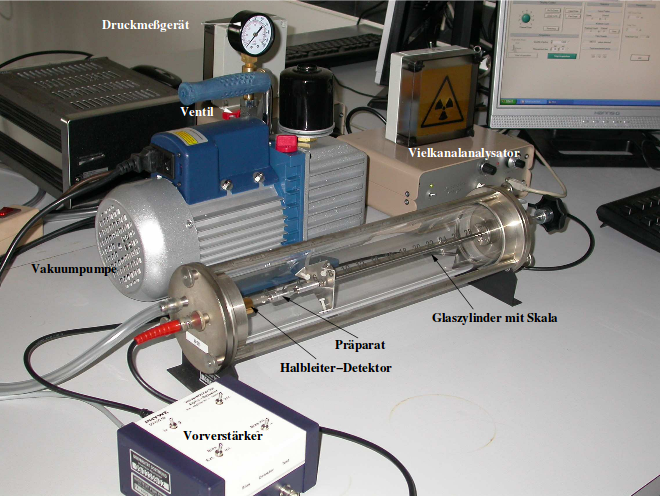
\includegraphics[height=7cm]{ressources/aufbau.png}
  \caption{Abbildung des verwendeten Versuchsaufbaus. \cite{skript}}
  \label{abb:1}
\end{figure}
Mithilfe einer Vakuumpumpe kann diese evakuiert werden, der Druckunterschied zum Atmosphärendruck wird an einem Manometer abgelesen.
Über die Schiene kann der Abstand der Strahlungsquelle zum Detektor fest gewählt werden.
Dieser Halbleiterdetektor ist in der Lage, sowohl die Anzahl der Impulse als auch die relative Energie der $\alpha$-Teilchen zu messen.
Die grundlegende Funktionsweise ist, dass durch die Strahlung Elektron-Loch-Paare entstehen, so dass freie Ladungen entstehen.
Diese werden an Elektroden registriert, und der vom Vorverstärker verstärkte Puls kann verarbeitet werden.
Im vorliegenden Versuchsaufbau wird diese Auswertung über das Computerprogramm Multichannel Analyzer realisiert.
Dieses bietet unter anderem die Möglichkeit, die Gesamtzählrate über einen festgelegten Zeitraum sowie eine Pulshöhenanalyse durchzuführen.
